\chapter{実験装置}
\section{プレーナートラップ}
本実験で使用する電極の写真を\Fig{Using_PlannerTrap}に示す.
\begin{figure}[h]
	\begin{center}
		\includegraphics[width = 0.6\linewidth]{./experimental_setup/figure/Using_PlannerTrap.png}
		\caption{本実験で使用するプレーナートラップ}
		\label{fig:Using_PlannerTrap}
	\end{center}
\end{figure}

\section{光学系}
\Fig{optical_system}にイオン捕獲のためのレーザーの光学系を示す.
\begin{figure}[h]
	\centering
		\includegraphics[width = 0.7\linewidth]{./experimental_setup/figure/Optical_System.png}
		\caption{プレーナートラップに照射するレーザーの光学系}
		\label{fig:optical_system}
\end{figure}

\section{レーザー}
\begin{table}[h]
	\centering
		\caption{$^{40}{\rm Ca}^+$を捕獲するときに使用するレーザーの波長}
		\label{tb:use_laser}
			\begin{tabular}{c|c} \hline \hline
				基準周波数 & 632 nm \\ 
				$^{40}{\rm Ca}$のイオン化 & 423 nm, 375 nm \\
				$^{40}{\rm Ca}^+$の冷却 & 397 nm \\
				$^{40}{\rm Ca}^+$のリポンプ & 866 nm \\ \hline 
			\end{tabular}
\end{table}
イオントラップに使用するレーザーのビーム径とその強度をスリット走査型光ビームプロファイラ(THORLABS,BP209-VIS/M)とデジタルパワー\&エネルギーメータ(THORLABS,PM100D)およびフォトダイオードパワーセンサー(THORLABS,S120C)を用いて計測を行った.
まず,各レーザーの強度を\Tb{AllLaserPower}に示す.

\begin{table}[h]
	\begin{center}
		\caption{各レーザーのパワー一覧表}
		\label{tab:AllLaserPower}
		\begin{tabular}{c|c} \hline \hline
			波長 (nm) & 強度 ($\mu$W) \\ \hline
			375 &4.1 \\ \hline
			397 &17.4 \\ \hline
			423 &28.4 \\ \hline
			866 &700 \\ \hline
		\end{tabular}
	\end{center}
\end{table}

次に,ビーム径の計測結果を\Fig{AllLaserBeamProfile}に示す.

\begin{figure}[h]
	\begin{center}
	\begin{minipage}{0.48\linewidth}
		\includegraphics[width = 0.98\columnwidth]{./experimental_setup/figure/AllLaserXpos.jpg}
	\end{minipage}
	\begin{minipage}{0.48\linewidth}
		\begin{center}
		\includegraphics[width = 0.98\columnwidth]{./experimental_setup/figure/AllLaserYpos.jpg}
		\end{center}
	\end{minipage}
	\caption{4種類のレーザーのx,y方向についてのビームプロファイル結果}
	\label{fig:AllLaserBeamProfile}
	\end{center}
\end{figure}

そして,得られたビームプロファイルにガウシアンによるフィッティングを行った様子を\Fig{GaussianFitting}に示し,その結果を\Tb{GaussianFitting}にまとめている.\\

\begin{table}[h]
	\begin{center}
		\caption{ビームプロファイラで得られた各ビームのプロファイルにガウシアンフィッティングをかけて得られたパラメータ}
		\label{tab:GaussianFitting}
		\begin{tabular}{c|cc|cc} \hline \hline
			波長 (nm)&位置(x) ($\mu$m)&ビーム径(x) ($\mu$m) &位置(y) ($\mu$m)& ビーム径(y) ($\mu$m)\\ \hline
			375&-2600.82$\pm$0.035&6.96$\pm$0.049&-1051.14$\pm$0.028&9.37$\pm$0.04 \\
			397&-2606.08$\pm$0.026&24.21$\pm$0.037&-1056.17$\pm$0.016&18.45$\pm$0.023 \\
			423&-2611.55$\pm$0.05&30.20$\pm$0.072&1042.25$\pm$0.03&39.85$\pm$0.054 \\
			866&-2606.08$\pm$0.138&77.20$\pm$0.196&-1054.24$\pm$0.06&54.72$\pm$0.085 \\\hline
		\end{tabular}
	\end{center}
\end{table}

\clearpage

\begin{figure}[h]
	\begin{center}
	%%%12
	\begin{minipage}{0.48\linewidth}
	\begin{center}
			\includegraphics[width = 0.98\columnwidth]{./experimental_setup/figure/375GaussianFittingXpos.jpg}
	\end{center}
	\end{minipage}
	\begin{minipage}{0.48\linewidth}
	\begin{center}
			\includegraphics[width=0.98\columnwidth]{./experimental_setup/figure/375GaussianFittingYpos.jpg}
	\end{center}
	\end{minipage}
	%%%34
	\begin{minipage}{0.48\linewidth}
	\begin{center}
		\includegraphics[width = 0.98\columnwidth]{./experimental_setup/figure/397GaussianFittingXpos.jpg}
	\end{center}
	\end{minipage}
	\begin{minipage}{0.48\linewidth}
	\begin{center}
		\includegraphics[width=0.98\columnwidth]{./experimental_setup/figure/397GaussianFittingYpos.jpg}
	\end{center}
	\end{minipage}
	%%%56
	\begin{minipage}{0.48\linewidth}
	\begin{center}
		\includegraphics[width = 0.98\columnwidth]{./experimental_setup/figure/423GaussianFittingXpos.jpg}
	\end{center}
	\end{minipage}
	\begin{minipage}{0.48\linewidth}
	\begin{center}
		\includegraphics[width=0.98\columnwidth]{./experimental_setup/figure/423GaussianFittingYpos.jpg}
	\end{center}
	\end{minipage}
	%%%78
	\begin{minipage}{0.48\linewidth}
	\begin{center}
		\includegraphics[width = 0.98\columnwidth]{./experimental_setup/figure/866GaussianFittingXpos.jpg}
	\end{center}
	\end{minipage}
	\begin{minipage}{0.48\linewidth}
	\begin{center}
		\includegraphics[width = 0.98\columnwidth]{./experimental_setup/figure/866GaussianFittingYpos.jpg}
	\end{center}
	\end{minipage}
	\caption{各波長に対してx,y方向それぞれのビームプロファイルにガウシアンフィッティングをかけた結果}
	\label{fig:GaussianFitting}
	\end{center}
\end{figure}

\section{電気系}